\input{slides_template}	% nothing to do here
\input{c_advanced_info} % TODO modify this if you have not already done so

% meta-information
\newcommand{\topic}{
	Advanced data structures
}

\usepackage{tikz}

% nothing to do here
\title{\topic}
\supertitle{\course}
\date{}

% the actual document
\begin{document}

\maketitle

\begin{frame}{Contents}
	\tableofcontents
\end{frame}

\begin{frame}
	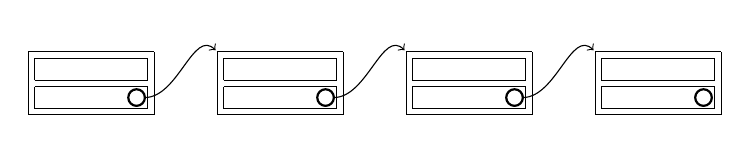
\begin{tikzpicture}[scale=.8]
		\draw (0,0) -- (0,1);
		\draw (0,0) -- (2,0);
		\draw (0,1) -- (2,1);
		\draw (2,0) -- (2,1);
		
		\draw (.1,.1) -- (.1,.45);
		\draw (.1,.1) -- (1.9,.1);
		\draw (.1,.45) -- (1.9,.45);
		\draw (1.9,.1) -- (1.9,.45);
		
		\node[circle, thick, draw=black, minimum size=6pt, inner sep = 0pt] at (1.72,.275) {};
		\draw (1.85,.275) edge[out=0,in=135,->,shorten >=.2ex] (3,1);
		
		\draw (.1,.55) -- (.1,.9);
		\draw (.1,.55) -- (1.9,.55);
		\draw (.1,.9) -- (1.9,.9);
		\draw (1.9,.55) -- (1.9,.9);
		
		
		\draw (3,0) -- (3,1);
		\draw (3,0) -- (5,0);
		\draw (3,1) -- (5,1);
		\draw (5,0) -- (5,1);
		
		\draw (3.1,.1) -- (3.1,.45);
		\draw (3.1,.1) -- (4.9,.1);
		\draw (3.1,.45) -- (4.9,.45);
		\draw (4.9,.1) -- (4.9,.45);
		\node[circle, thick, draw=black, minimum size=6pt, inner sep = 0pt] at (4.72,.275) {};
		\draw (4.85,.275) edge[out=0,in=135,->,shorten >=.2ex] (6,1);
		
		
		\draw (3.1,.55) -- (3.1,.9);
		\draw (3.1,.55) -- (4.9,.55);
		\draw (3.1,.9) -- (4.9,.9);
		\draw (4.9,.55) -- (4.9,.9);
		
		
		\draw (6,0) -- (6,1);
		\draw (6,0) -- (8,0);
		\draw (6,1) -- (8,1);
		\draw (8,0) -- (8,1);
		
		\draw (6.1,.1) -- (6.1,.45);
		\draw (6.1,.1) -- (7.9,.1);
		\draw (6.1,.45) -- (7.9,.45);
		\draw (7.9,.1) -- (7.9,.45);
		\node[circle, thick, draw=black, minimum size=6pt, inner sep = 0pt] at (7.72,.275) {};
		\draw (7.85,.275) edge[out=0,in=135,->,shorten >=.2ex] (9,1);
		
		\draw (6.1,.55) -- (6.1,.9);
		\draw (6.1,.55) -- (7.9,.55);
		\draw (6.1,.9) -- (7.9,.9);
		\draw (7.9,.55) -- (7.9,.9);
		
		
		\draw (9,0) -- (9,1);
		\draw (9,0) -- (11,0);
		\draw (9,1) -- (11,1);
		\draw (11,0) -- (11,1);
		
		\draw (9.1,.1) -- (9.1,.45);
		\draw (9.1,.1) -- (10.9,.1);
		\draw (9.1,.45) -- (10.9,.45);
		\draw (10.9,.1) -- (10.9,.45);
		\node[circle, thick, draw=black, minimum size=6pt, inner sep = 0pt] at (10.72,.275) {};
		
		\draw (9.1,.55) -- (9.1,.9);
		\draw (9.1,.55) -- (10.9,.55);
		\draw (9.1,.9) -- (10.9,.9);
		\draw (10.9,.55) -- (10.9,.9);
		
	\end{tikzpicture}
\end{frame}

% nothing to do from here on
\end{document}
